\documentclass{article}
\usepackage{verbatim}
\usepackage{amsfonts}
\usepackage{geometry}
\usepackage{amsmath}
\usepackage{amsthm}
\usepackage{amssymb}
\usepackage{listings}
\usepackage{ctex}
\usepackage{graphicx}
\usepackage{clrscode3e}
\usepackage{txfonts}
\usepackage{fontspec}
\usepackage{float}
\usepackage{enumerate}
\usepackage{subfigure}
\setmainfont{Times New Roman}
\geometry{top=2.5cm,bottom=2.5cm,left=2.5cm,right=2.5cm}
\setlength\parindent{0em}
\begin{document}
	\subsection*{4.3.6.6 KP的dual PTAS}
	解法思路:使用\proc{Bin-P}\par 
	\begin{enumerate}[Step 1:]
		\item 距离函数:
		$$h(I,T)=\max \left\{\frac{\sum_{i\in T}w_i-b}{nb},0\right\}$$
		\item s-KP: $I=\left\{q_1,q_2,\dots,q_s,b,n_1,n_2,\dots,n_s,c_1,c_2,\dots, c_n\right\}$
		\item DP-KPs: $(m_1,m_2,\dots,m_s)\in \left\{0,\dots,n_1\right\}\times \left\{0,\dots,n_2\right\}\times \cdots \times \left\{0,\dots,n_2\right\}$
		\begin{enumerate}[1.]
			\item $DP(m_1,m_2,\dots,m_s,d)=\max\left\{DP(m_1,\dots,m_i-1,\dots,m_s,d-q_i)+c_{i_1}\right\}$
			\item 
			可以穷举所有的满足背包容量的选择,即$\sum_{i=1}^{s}m_iq_i\le b$。然后计算它们的代价,$\forall i\le s$,$n_i$个物品中$m_i$个价值最大的被使用。
		\end{enumerate}
	穷举的代价为$O(n_1\cdot n_2\cdot\ \cdots\ \cdot n_s)\le O\left(\left(n/s\right)^s\right)$
	\item 
	KP-PTA$\epsilon$和KP-PTAS\par 
	令$s=[1/\epsilon],l_i=0$且$l_i=(i-1)\epsilon b,l_{s+1}=b$\par 
	通过rounding得到$I'=\left\{l_1,l_2,\dots,l_n,b,n_1,n_2,\dots,n_s,c_1,c_2,\dots,c_n\right\}$,对$I'$使用DP-KPs
	\begin{enumerate}[1.]
		\item 时间复杂度$O\left((n\epsilon)^{1/\epsilon}\right)$
		\item $cost(KP-PTAS(I,\epsilon))=cost(DP-KPs(I'))\ge Opt_{KP}(I)$,因为物品的重量减少了(现在能装入更多的物品)
		\item $\forall i\in T,w_i-w_i'\le \epsilon b$且$\sum_{i\in T}w_i'\le b$
		$$h(I,T)=\max \left\{\frac{\sum_{i\in T}w_i-b}{nb}, 0\right\}\le \frac{\sum_{i\in T}(w_i'+\epsilon b)-b}{nb}\le \frac{b+n\epsilon b-b}{nb}=\epsilon$$
	\end{enumerate}
	\end{enumerate}
	\subsection*{5.3.3.9}
	\begin{enumerate}[(i)]
		\item 
		\[
		Jac\left[\frac{ab}{n}\right]=\prod_{i=1}^{l}\left((ab)^{(p_i-1)/2}\mod p_i\right)=\prod_{i=1}^{l}\left(a^{(p_i-1)/2}\mod p_i\right)\prod_{i=1}^{l}\left(b^{(p_i-1)/2}\mod p_i\right)=Jac\left[\frac{a}{n}\right]Jac\left[\frac{b}{n}\right]
		\]
		\item 若$a\equiv b\mod p$,则$a\equiv b\mod q$,其中$q$是$p$的某个因数:
		\[
		Jac\left[\frac{a}{n}\right]=\prod_{i=1}^{l}\left(a^{(p_i-1)/2}\mod p_i\right)=\prod_{i=1}^{l}\left(b^{(p_i-1)/2}\mod p_i\right)=Jac\left[\frac{b}{n}\right]
		\]
		\item 本题的重点是需要用到"quadratic reciprocity",使得$Leg[p/q]$和$Leg[q/p]$能够建立关系。\par 
		令$n=p_1^{k_1}p_2^{k_2}\cdots p_l^{k_l}, a=q_1^{r_1}q_2^{r_2}\cdots q_m^{r_m}$,其中$p_1,p_2,\cdots,p_l,q_1,q_2,\cdots, q_m$为成对的不同奇质数,由$Jac$和$Leg$符号的定义,可得:
		\[
		Jac\left[\frac{a}{n}\right]=\prod_{i=1}^{l}\left(Leg\left[\frac{a}{p_i}\right]\right)^{k_i}=\prod_{i=1}^{l}\prod_{j=1}^{m}\left(Leg\left[\frac{q_j}{p_i}\right]\right)^{k_ir_j}
		\]
		再由\emph{law of quadratic reciprocity}, 即$Leg[p/q]Leg[q/p]=(-1)^{\frac{p-1}{2}\frac{q-1}{2}}$,其中$p,q$为不同的奇质数,由二项式定理:
		\[
		\begin{aligned}
			\frac{n-1}{2}&=\frac{\prod_{i=1}^{l}p_i^{k_l}-1}{2}\\
			&=\frac{\prod_{i=1}^{l}\left(2\cdot \frac{p_i-1}{2}+1\right)^{k_l}-1}{2}\\
			&\equiv\frac{\prod_{i=1}^{l}\left(2k_i\cdot \frac{p_i-1}{2}+1\right)-1}{2}\mod 2\\
			&\equiv\sum_{i=1}^{l}k_i\left(\frac{p_i-1}{2}\right)\mod 2\\
			\therefore Jac\left[\frac{a}{n}\right]&=\prod_{i=1}^{l}\prod_{j=1}^{m}\left(Lef\left[\frac{q_j}{p_i}\right]\right)^{k_ir_j}\\
			&=\prod_{i=1}^{l}\prod_{j=1}^{m}\left(Lef\left[\frac{q_j}{p_i}\right]\right)^{k_ir_j}\left(-1\right)^{k_i\frac{p_i-1}{2}r_j\frac{q_i-1}{2}}\\
			&=\left(-1\right)^{\left(\sum_{i=1}^{l}k_i\frac{p_i-1}{2}\right)\left(\sum_{j=1}^{m}r_i\frac{q_i-1}{2}\right)}\prod_{i=1}^{l}\prod_{j=1}^{m}\left(Leg\left[\frac{p_i}{q_j}\right]\right)^{k_ir_j}\\
			&=\left(-1\right)^{\frac{a-1}{2}\frac{n-1}{2}}Jac\left[\frac{n}{a}\right]
		\end{aligned}
		\]
		\item 显然
		\[
		Jac\left[\frac{1}{n}\right]=\prod_{i=1}^{l}\left(Leg\left[\frac{1}{p_i}\right]\right)^{k_1}=1
		\]
		\item 使用quadratic reciprocity的第二补式:
		\[
		Leg\left[\frac{2}{p}\right]=(-1)^{\frac{p^2-1}{8}}=\left\{
		\begin{array}{cl}
		-1,&p\equiv 3,5\mod 8\\
		1,&p\equiv 1,7\mod 8
		\end{array}
		\right.
		\]
		由$Jac$符号的定义:
		\[
		Jac\left[\frac{2}{n}\right]=\prod_{i=1}^{l}\left(Leg\left[\frac{2}{p_i}\right]\right)^{k_i}=\prod_{i=1}^{l}\left((-1)^{\frac{p_i^2-1}{8}}\right)^{k_i}
		\]
		再次使用二项式定理:
		\[
		\begin{aligned}
			\frac{n^2-1}{8}&=\left(\left(\prod_{i=1}^{l}p_i^{k_i}\right)^2-1\right)\Big /8\\
			&=\cfrac{\prod_{i=1}^{l}\left(8\frac{p_i^2-1}{8}+1\right)^{k_i}-1}{8}\\
			&\equiv\cfrac{\prod_{i=1}^{l}\left(8k_i\frac{p_i^2-1}{8}+1\right)-1}{8}\mod 2\\
			&\equiv \sum_{i=1}^{l}k_i\frac{p_i^2-1}{8}\mod 2\\
			\therefore Jac\left[\frac{2}{n}\right]&=\prod_{i=1}^{l}\left(Leg\left[\frac{2}{p_i}\right]\right)^{k_i}=\prod_{i=1}^{l}\left((-1)^{\frac{p_i^2-1}{8}}\right)^{k_i}
		\end{aligned}
		\]
		\[
		\\
		=(-1)^{\sum_{i=1}^{l}k_i\frac{p_i^2-1}{8}}=(-1)^{\frac{n^2-1}{8}}=\left\{
		\begin{array}{cl}
		-1,&n\equiv 3,5\mod 8\\
		1,&n\equiv 1,7\mod 8
		\end{array}
		\right.
		\]
		\subsection*{5.3.3.10}
		\begin{codebox}
			\zi \proc{Jacob$(a,n)$}\Comment{假定$a$和$n$互质}\li 
			\If \id{a} is even\Comment{(v),(i)}\Then\li 
			\If $n\equiv 3,5\mod 8$\Then\li 
			\Return $-\proc{Jacob(a/2,n)}$\li  
			\Else\li 
			\Return $\proc{Jacob(a/2,n)}$\End\End \li 
			\If $a==1$\Then\li 
			\Return 1\Comment{(iv)}\End\li 
			\If $(a\ \&\ 0x2==1)\ \&\&\ (b\ \&\ 0x2==1)$\Then\li 
			\Return -\proc{Jacob$(n\mod a,a)$}\li   
			\Else\li 
			\Return \proc{Jacob$(n\mod a,a)$}
		\end{codebox}
	\end{enumerate}
	\subsection*{3.3.2.9}
	Set cover problem. $Pot(X)$ is the set of all subsets of the set $X$. Similar to \proc{VCP}, use divide-and-conquer.\par 
	Divide: $((X_i,F_i),k-1)$: Select any $S_i\in F$. Let $X_i=X\backslash S_i,F_i=f(F,i)$, function $f$ deletes $S_i$ and all elements of $S_i$ in $S_1,\cdots,S_{i-1},S_{i+1},\cdots, S_l$. Using induction, $((X_T,F_T),0)$ is trivial. Complexity is $O(Pat^{pat}|X|)$.
	\subsection*{不必限制输入的网络流算法}
	改变算法3.2.3.10的第3步和第4步:
	\begin{enumerate}[1.]
		\item \emph{Edmonds-Karp algorithm}: 通过BFS找到最短路
		\item \emph{Dinic's blocking flow algorithm}: 在residual graph上使用BFS构造一个分层图
	\end{enumerate}
	\subsection*{branching-and-bound解背包问题}
	\proc{Knapsack Problem}: KP$\left(b,\left\{w_1,w_2,\cdots,w_n\right\},\left\{c_1,c_2,\cdots,c_n\right\}\right)$
	\begin{enumerate}[(1)]
		\item 建立一个backtracking tree. 在树的每个内部节点,根据物品是否放入背包来选择分支
		\item 剪枝和BFS/DFS,设当前可行解的价值$cost=c$
		\begin{enumerate}[i.]
			\item $\sum w_{k_i}>b$
			\item 当前的价值为$a$,当前的总重量$weight=d$,当前还能放入的且性价比$(c_i/w_i)$最高的物品为$q$,若$a+(b-d)\cdot q<c$,则剪枝
		\end{enumerate}
		\item 有利的输入:最开始就找到了最优解,同样的剪枝策略被不断使用;不利输入:难以剪枝 
	\end{enumerate}
	\subsection*{3.4.2.1}
	\begin{figure}[H]
		\centering
		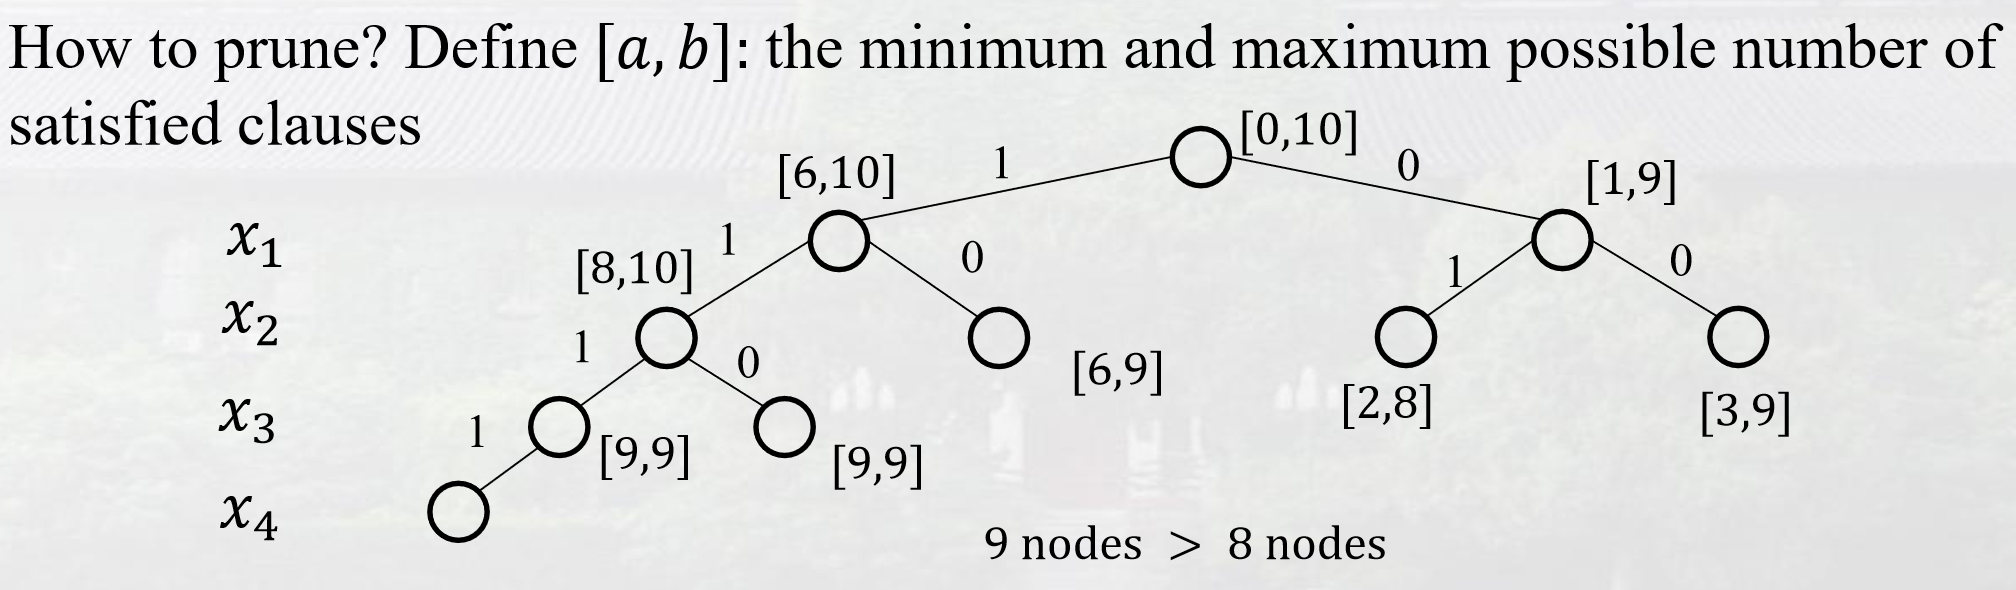
\includegraphics[width=1\linewidth]{hw4-2.png}
		\caption{Ex 3.4.2.1中的搜索树}
	\end{figure}
	\subsection*{3.4.2.2}
	\begin{figure}[H]
		\begin{minipage}[t]{0.5\linewidth}
			\centering
			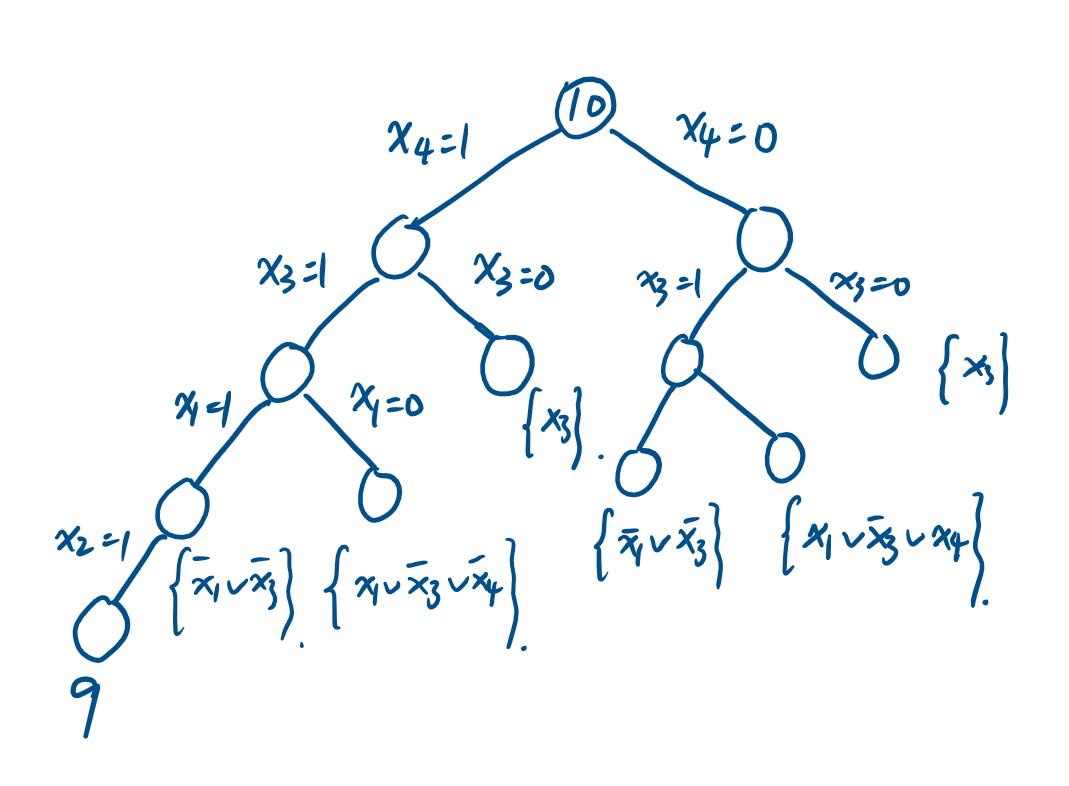
\includegraphics[width=3in]{ex4-2.jpg}
			\caption{右DFS}
		\end{minipage}%
		\begin{minipage}[t]{0.5\linewidth}
			\centering
			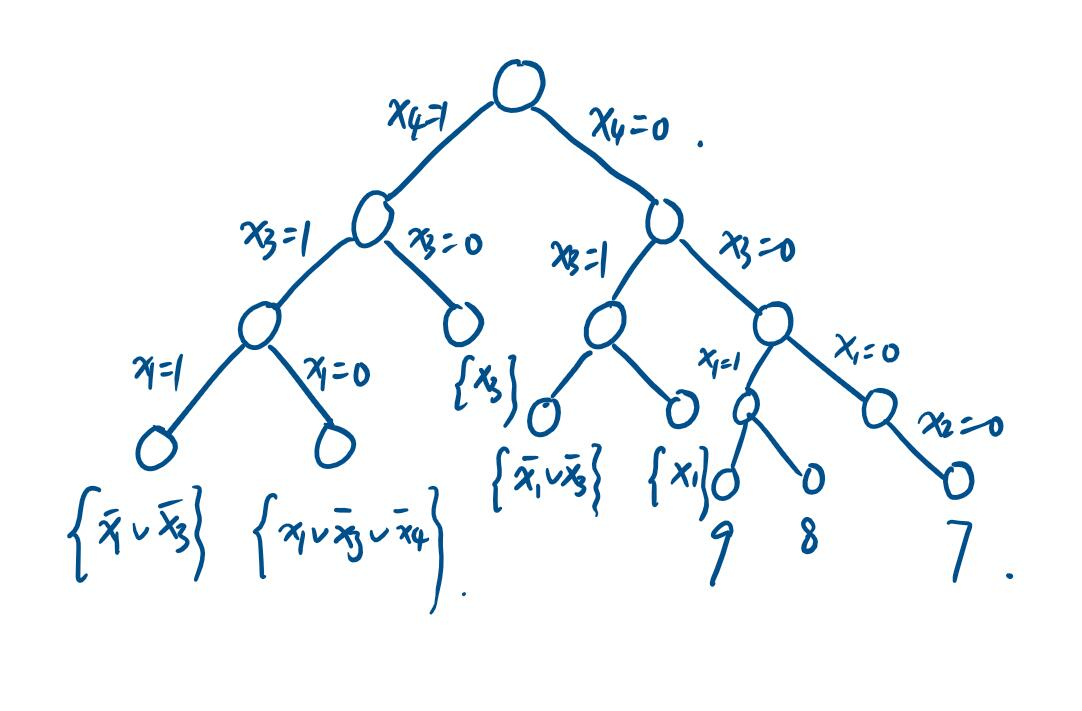
\includegraphics[width=3in]{ex4-3.jpg}
			\caption{左DFS}
		\end{minipage}
	\end{figure}
\end{document}